\documentclass[tikz,border=4pt]{standalone}
\usepackage{amsmath}
\begin{document}
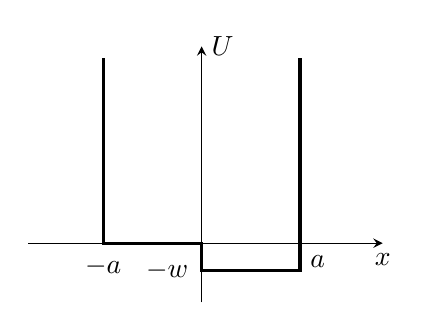
\begin{tikzpicture}[>=stealth, thick, scale=1.0]
  % Axes
  \draw[->, line width=0.5pt] (-2.2, 0) -- (2.3, 0) node[below] {$x$};
  \draw[->, line width=0.5pt] (0, -0.75) -- (0, 2.5) node[right] {$U$};

  % Step-perturbed infinite well: U = 0 (-a < x <= 0), U = -w (0 < x < a)
  \draw[line width=1.1pt] (-1.25, 2.35) -- (-1.25, 0) -- (0, 0) -- (0, -0.35) -- (1.25, -0.35) -- (1.25, 2.35);

  % Labels
  \node[below] at (-1.25, -0.05) {$-a$};
  \node[below right] at (1.25, -0.02) {$a$};
  \node[left] at (-0.04, -0.35) {$-w$};
\end{tikzpicture}
\end{document}
